\documentclass[conference]{IEEEtran}
\IEEEoverridecommandlockouts
% The preceding line is only needed to identify funding in the first footnote. If that is unneeded, please comment it out.
\usepackage{cite}
\usepackage{amsmath,amssymb,amsfonts}
\usepackage{algorithmic}
% \usepackage[ruled,vlined]{algorithm2e}
\usepackage{graphicx}
\usepackage{textcomp}
\def\BibTeX{{\rm B\kern-.05em{\sc i\kern-.025em b}\kern-.08em
    T\kern-.1667em\lower.7ex\hbox{E}\kern-.125emX}}
\begin{document}

\title{Poisson Multi-Bernoulli Filter for Extended Object Estimation\\
% {\footnotesize \textsuperscript{*}Note: Sub-titles are not captured in Xplore and
% should not be used}
% \thanks{Identify applicable funding agency here. If none, delete this.}
}

\author{\IEEEauthorblockN{1\textsuperscript{st} Yuxuan Xia}
\IEEEauthorblockA{\textit{Department of Electrical Engineering} \\
\textit{Chalmers University of Technology}\\
G\"{o}teborg, Sweden \\
yuxuanx@student.chalmers.se}
\and
\IEEEauthorblockN{2\textsuperscript{nd} Karl Granstr\"{o}m}
\IEEEauthorblockA{\textit{Department of Electrical Engineering} \\
\textit{Chalmers University of Technology}\\
G\"{o}teborg, Sweden \\
karl.granstrom@chalmers.se}
\and
\IEEEauthorblockN{3\textsuperscript{rd} Lennart Svensson}
\IEEEauthorblockA{\textit{Department of Electrical Engineering} \\
\textit{Chalmers University of Technology}\\
G\"{o}teborg, Sweden \\
lennart.svensson@chalmers.se}
}

\maketitle

\begin{abstract}
In this paper, a Poisson multi-Bernoulli (PMB) filter for multiple extended targets estimation is presented. The PMB filter is based on the Poisson multi-Bernoulli mixture (PMBM) conjugate prior and approximates the multi-Bernoulli mixture (MBM) in the posterior as a single multi-Bernoulli. Different methods to merge the MBM are presented, along with their gamma Gaussian inverse Wishart implementation. The performance of the PMB filter is compared to the PMBM filter and the Probability Hypothesis Density filter in different simulated scenarios. 
\end{abstract}

\begin{IEEEkeywords}
multiple target tracking, extended target, random matrix model, random finite sets, Bayesian estimation, variational inference
\end{IEEEkeywords}

\section{Introduction}
% The development of autonomous driving has attracted an enormous amount of interest in research during last decades. In order for an autonomous vehicle to be deployed in real-world environments, it must be capable of reliably and efficiently modelling static as well as dynamical obstacles, e.g., landmarks, pedestrians and other nearby moving vehicles. 
Multiple target tracking (MTT) denotes the process of estimating the set of target trajectories based on a sequence of noise-corrupted measurements including missed detections and false alarms. Traditionally, MTT algorithms have been tailored with the ``point target'' assumption that each target is modelled as a point without spatial extent and that each target gives rise to at most one measurement per time scan. However, the high-resolution feature of modern radar and lidar sensors makes the “point target” assumption unrealistic since it is common that a target may occupy several sensor resolution cells. The tracking of such a target leads to the so-called extended target tracking problem, and the objective is to recursively determine the extent and kinematic parameters of the target over time. In this paper, we only focus on the estimation of the current set of targets, which refers to multiple target filtering. 

In extended target tracking, a non-standard measurement model is needed to model the number and the spatial distribution of generated measurements for each target. A common choice for modelling the number of measurements is the inhomogeneous Poisson Point Process (PPP), proposed in \cite{ppp}. As for the modelling of the spatial distribution, two popular models are the Random Hyper-surface Models \cite{hypersurface} and the Gaussian inverse Wishart (GIW) approach \cite{randomMatrix,randomMatrix2}. The former is designed for general star-convex shape; the latter relies on the elliptic shape that it models the spatial distribution of target-generated measurements as Gaussian with unknown mean and covariance. The Gamma GIW (GGIW) model \cite{phdextended,cphdextended} is an extension of the GIW model by incorporating the estimation of target measurement rates.

Solving the MTT problem is mainly complicated by the unknown correspondence between targets and measurements, known as data association. Because each target can generate multiple measurements per time scan, the problem of data association can be even more challenging in multiple extended target tracking. Many of the existing multiple extended target tracking algorithms are based on random finite sets (RFS) \cite{rfs} with the distribution of target-generated measurements modelled as GIW or GGIW, such as the Probability Hypothesis Density (PHD) filter \cite{phdextended2,phdextended3}, the Cardinalised PHD (CPHD) filter \cite{cphdextended}, the Labelled Multi-Bernoulli filters (GLMB and LMB) \cite{lmbextended}, and the Poisson Multi-Bernoulli Mixture (PMBM) filter \cite{pmbmextended,pmbmextended2}. The PHD and CPHD filters are based on moment approximations of posterior distributions, while the GLMB filter and the PMBM filter are based on conjugate priors that can provide accurate approximations to the exact posterior distributions. 

A variational Bayesian approach to approximating the PMBM density with a single Poisson multi-Bernoulli (PMB) was presented in \cite{variational} for point target tracking. The performance evaluation of filters based on multi-Bernoulli (MB) conjugate prior for point target estimation given in \cite{performanceevaluation} has shown that the PMB filter has the best overall performance regarding estimation error and computational time, but it is not yet clear how the variational method proposed in \cite{variational} can be used on extended target tracking. The main contribution of this paper is presenting the PMB filter for multiple extended target estimation, along with its GGIW implementation. Two different implementations of the variational MB algorithm for merging MBM describing already detected targets are studied, one is based on the efficient approximation of feasible set proposed in \cite{variational}, and the other is based on the optimal assignment following a similar optimisation procedure used by the set joint probabilistic data association (SJPDA) filter \cite{sjpda}. In addition, we propose a method to merge the MBM describing newly detected target in a reasonable way. 

The paper is organised as follows. Background on multiple extended target tracking is given in Section II. The PMB filter and its GGIW implementation are presented in Section III and IV. Simulation results are presented in Section V.

\section{Background}
In this section, we first give some background on Bayesian filtering and RFS modelling. Next, the standard target transition model and extended target measurement model used in this work are outlined. At last, we review the PMBM conjugate prior and data association. 

\begin{table}[!t]
\footnotesize
\caption{Notations}
\label{tab:notations}
\centering
% \resizebox{\textwidth}{!}{%
\begin{tabular}{l}
  \hline
  \begin{minipage}{0.45\textwidth}
    \vskip 1pt
    \begin{itemize}
    \item $\langle a,b\rangle=\int a(x)b(x)$: inner product of $a(x)$ and $b(x)$.
    \item $|V|$: determinant of matrix $V$.
    \item $|\mathbf{X}|$: cardinality of set $\mathbf{X}$.
   \item $\Pi_N$: set of permutation functions on $I_N \triangleq \{1,...,N\}$
   $$\Pi_N = \{\pi:I_N\rightarrow I_N|i\neq j\Rightarrow \pi(i)\neq\pi(j)\}.$$
   \item $\uplus$: disjoint set union, i.e., $Y\uplus U=X$ means that $Y\cup U=X$ and $Y\cap U=\emptyset$.
   \item $\text{KL}(p||q)=\int p(x)\log\bigg(\frac{p(x)}{q(x)}\bigg)dx$: KullBack-Leibler divergence between $p(x)$ and $q(x)$.
   \item $\Gamma_d(\cdot)$: multivariate gamma function.
   \item $\varphi_0(\cdot)$: digamma function.
   \item $\text{Tr}(X)$: trace of matrix $X$.
   \item $\mathbf{I}_m$: identity matrix of size $m\times m$.
   \end{itemize}
   \vskip 1pt
 \end{minipage}
 \\
  \hline
 \end{tabular}
\end{table}

\subsection{Bayesian multi-object filtering}

In RFS-based MTT methods, target states and measurements are represented in the form of finite sets. Let $\mathbf{x}_k$ denote the single target state at discrete time step $k$, and let $\mathbf{X}_k$ denote the target set. The target set cardinality $|\mathbf{X}_k|$ is a time-varying discrete random variable, and each target state $\mathbf{x}_k\in\mathbf{X}_k$ is also a random variable. The set of measurements obtained at time step $k$ is denoted as $\mathbf{Z}_k$, including clutter and target-generated measurements with unknown origin. The sequence of all the measurement sets received so far up to time step $k$ is denoted as $\mathbf{Z}^k$. More notations are given in Table \ref{tab:notations}.

The objective of multiple target filtering is to estimate the set of targets $\mathbf{X}_k$, including the number of targets and individual target state, using the information contained in the measurement set sequence $\mathbf{Z}^k$. In extended target tracking, the target state models both kinematic properties and target extent. Let $f_{k|k}(\mathbf{X}_k|\mathbf{Z}^k)$, $f_{k+1,k}(\mathbf{X}_k|\mathbf{Z}^k)$ and $f_k(\mathbf{Z}_k|\mathbf{X}_k)$ denote the multi-target set density, the multi-target transition density and the multi-target measurement likelihood respectively. The multi-target Bayes filter propagates in time the multi-target set density $f_{k-1|k-1}(\mathbf{X}_{k-1}|\mathbf{Z}^{k-1})$ using the Chapman-Kolmogorov prediction
\begin{multline}
f_{k|k-1}(\mathbf{X}_k|\mathbf{Z}^{k-1}) \\= \int f_{k,k-1}(\mathbf{X}_k|\mathbf{X}_{k-1})f_{k-1|k-1}(\mathbf{X}_{k-1}|\mathbf{Z}^{k-1})\delta \mathbf{X}_{k-1},
\end{multline}
and then updates the density using the Bayes update
\begin{equation}
f_{k|k}(\mathbf{X}_k|\mathbf{Z}^k) = \frac{f_{k}(\mathbf{Z}_k|\mathbf{X}_k)f_{k|k-1}(\mathbf{X}_k|\mathbf{Z}^{k-1})}{\int f_{k}(\mathbf{Z}_k|\mathbf{X}_k)f_{k|k-1}(\mathbf{X}_k|\mathbf{Z}^{k-1})\delta \mathbf{X}_k},
\end{equation}
where the set integral is defined in \cite[Sec 11.3.3]{rfs}.

\subsection{Random set modelling}
Two basic forms of RFS distribution used in this work are the PPP and the Bernoulli process. A PPP is an RFS whose cardinality is Poisson distributed, and each target is independent and identically distributed (i.i.d.). The PPP intensity $D(\mathbf{x})=\mu f(\mathbf{x})$ is determined by the scalar Poisson rate $\mu$ and the spatial distribution $f(\mathbf{x})$. The PPP density is given by
\begin{equation}
f(\mathbf{X}) = e^{-\mu}\prod_{\mathbf{x}\in\mathbf{X}}\mu f(\mathbf{x}).
\label{eq:ppp}
\end{equation}
A Bernoulli process with probability of existence $r$ and existence-conditioned probability density function (PDF) $f(\mathbf{x})$ has RFS density
\begin{equation}
f(\mathbf{X}) = \begin{cases}
    1-r& \mathbf{X}=\emptyset\\
    r\cdot f(\mathbf{x})& \mathbf{X}=\{\mathbf{x}\}\\
    0& \text{otherwise},
\end{cases}
\label{eq:bernoulli}
\end{equation}
where the cardinality $|\mathbf{X}|$ is Bernoulli distributed with parameter $r\in[0,1]$. The Bernoulli process offers a convenient way to capture both the uncertainty regarding the target existence and state. In MTT, targets are typically assumed to be independent. Thus, multiple targets can be represented as an MB RFS $\mathbf{X}$, which is a disjoint union of independent Bernoulli RFSs $\mathbf{X}^i$, i.e., $\mathbf{X}=\uplus_{i\in\mathbb{I}} \mathbf{X}^i$, where $\mathbb{I}$ is an index set. The RFS density of an MB process can be represented as 
\begin{equation}
f(\mathbf{X}) = 
\begin{cases}
\sum_{\uplus_{i\in\mathbb{I}}\mathbf{X}^i=\mathbf{X}}\prod_{i\in\mathbb{I}}f^i(\mathbf{X}^i), & |\mathbf{X}| \leq |\mathbb{I}| \\
0, & |\mathbf{X}| > |\mathbb{I}|
\end{cases}
\end{equation}
The MB distribution can be defined entirely by the parameters $\{r^i,f^i(\cdot)\}_{i\in\mathbb{I}}$ of the involved Bernoulli RFSs.

\subsection{Standard extended target measurement model}
The set of measurements $\mathbf{Z}_k$ is the union of a set of clutter measurements and sets of target-generated measurements. The clutter is modelled as a PPP with Poisson rate $\lambda$ and spatial distribution $c(\mathbf{z})$, independent of targets and any target-generated measurements. Each extended target may give rise to multiple measurements with a state dependent detection probability $p^D(\mathbf{x})$. If the extended target is detected, the target-generated measurements are modelled as a PPP with Poisson rate $\gamma(\mathbf{x})$ and spatial distribution $\phi(\mathbf{z}|\mathbf{x})$, independent of all other targets and their corresponding generated measurements. The extended target set measurement likelihood for a nonempty set of measurements $\mathbf{Z}$ is the product of target detection probability and the PPP density of target-generated measurements \cite{pmbmextended2}
\begin{equation}
    \ell_{\mathbf{Z}}(\mathbf{x}) = p^D(\mathbf{x})e^{-\gamma(\mathbf{x})}\prod_{\mathbf{z}\in \mathbf{Z}}\gamma(\mathbf{x})\phi(\mathbf{z}|\mathbf{x}).
    \label{eq:extendedlikelihood}
\end{equation}
For an extended target state $\mathbf{x}$, the effective detection probability is the product of the target detection probability and the probability that the target generates at least one measurement, which is $1-e^{-\gamma(\mathbf{x})}$. Then the effective probability of missed detection can be calculated accordingly as
\begin{equation}
    q^D(\mathbf{x}) = 1 - p^D(\mathbf{x}) + p^D(\mathbf{x})e^{-\gamma(\mathbf{x})},
\end{equation}
which is also the measurement likelihood for an empty measurement set.

\subsection{Standard target transition model}
In this work, it is assumed that targets arrive according to a PPP, independently of any pre-existing targets. At each time step, target remains with a probability of survival $p^S_k(\mathbf{x})$. Targets depart according to i.i.d. Markov processes with probability $1-p^S_k(\mathbf{x})$. Target state at next time step only depends on its current state. Targets evolve independently according to i.i.d. Markov process with transition density $f_{k+1,k}(\mathbf{x}_{k+1}|\mathbf{x}_{k})$. 

\subsection{PMBM conjugate prior}
The PMBM conjugate prior for multiple extended target filtering was developed in \cite{pmbmextended,pmbmextended2}. In the PMBM filter, the target set is the union of two disjoint sets of undetected targets $\mathbf{X}^u$ and detected objects $\mathbf{X}^d$, i.e., $\mathbf{X} = \mathbf{X}^u\uplus\mathbf{X}^d$. The distribution of targets that have not been detected yet $\mathbf{X}^u$ is described by a PPP, while the distribution of targets that have been detected at least once $\mathbf{X}^d$ is described by an MBM, which is a normalized weighted sum of MB densities. The PMBM density is defined entirely by the parameters,
\begin{equation}
D^u, \{(\mathcal{W}^j,\{r^{j,i},f^{j,i}(\cdot)\}_{i\in\mathbb{I}^j})\}_{j\in\mathbb{J}},
\label{eq:update}
\end{equation}
where $D^u(\cdot)$ is the PPP intensity of the set of undetected targets, $\mathbb{I}^j$ is the index set of Bernoulli components in the $j$th MB, $r^{j,i}$ and $f^{j,i}(\cdot)$ are the existence probability and existence-conditioned PDF of the $i$th Bernoulli process in the $j$th MB, and $\mathcal{W}^j$ is the weight of the $j$th MB.


\subsection{PMBM data association}
The PMBM form is preserved by prediction and update. Each MB corresponds to a unique \textit{global hypothesis} for the detected targets, i.e., a particular history of data associations for all detected targets. Given a predicted PMBM density, for each predicted global hypothesis there are multiple possible data associations, each of which will result in an MB component in the updated MBM. A data association event includes a partitioning of measurement set $\mathbf{Z}$ into disjoint small subsets $\mathbf{C}$, called measurement cells, and an assignment of each measurement cell to a pre-existing target or the background (clutter or new target). 

Global hypotheses are made up of \textit{single target hypotheses}, each of which can represent the event that a pre-existing target is updated with a measurement cell, the event that a pre-existing target is not detected and the event that it is the first detection of the background, via a Bernoulli process. A \textit{track} is defined as a collection of single target hypotheses corresponding to the same target that was first detected. As a consequence, a new track is created for each measurement cell. If the measurement cell is associated with a pre-existing track, the new track would have existence probability equal to zero. A complexity analysis of the data association problem given in \cite{pmbmextended2} has shown that the number of MB distributions grows very rapidly over time. Approximations of the data association problem have been presented in \cite{pmbmextended2,soextended}, which can keep the number of global hypotheses at a tractable level. In this work, we focus on approximating the MBM as a single MB after solving the data association problem. 


\section{Poisson Multi-Bernoulli Filter}
In the PMB filter, the PMB density is preserved in the prediction step, whereas in the update step the posterior first becomes a PMBM density due to data association, then it is approximated as a PMB afterwards. In this section, the prediction and update steps of the PMB filter are presented. We then discuss approximation methods that result in a PMB posterior. The time index is omitted for brevity. 

\subsection{PMB filter recursion}
Given a posterior PMB density with parameters
\begin{equation}
D^u, {(r^i ,f^i(\cdot) )}_{i\in\mathbb{I}},
\end{equation}
and the standard dynamical model, the predicted density is a PMB density with parameters
\begin{equation}
D^u_+, {(r_+^i ,f_+^i(\cdot) )}_{i\in\mathbb{I}},
\label{eq:prediction}
\end{equation}
where 
\begin{subequations}
\begin{align}
    D^u_+(\mathbf{x}) &= D^b_+(\mathbf{x})+\langle D^u,p^Sf_{k+1,k}\rangle,\\
    r^i_+ &= \langle f^i,p^S\rangle r^i,\\
    f_+^i(\mathbf{x}) &= \frac{\langle f^i,p^Sf_{k+1,k}\rangle}{\langle f^i,p^S\rangle},
\end{align}
\end{subequations}
and $D^b(\cdot)$ denotes the PPP birth intensity. Detail derivation can be found in \cite{pmbmpoint}. 

Given a prior PMB density with parameters (\ref{eq:prediction}), a set of measurements $\mathbf{Z}$, and the standard measurement model, the updated density before the MBM merging is a PMBM (\ref{eq:update}). The updated PPP intensity is $D^u(\mathbf{x}) = q^D(\mathbf{x})D_+^u(\mathbf{x})$. For tracks continuing from previous time steps $i\in\mathbb{I}$, a hypothesis can be included as a missed detection or an update using a measurement cell $\mathbf{C}$. For missed detection hypotheses ($i\in\mathbb{I}$), the Bernoulli densities have parameters
\begin{subequations}
\begin{align}
    r^{j,i} &= \frac{r^i_+\langle f_+^i,q^D\rangle}{1-r_+^i+r^i_+\langle f_+^i,q^D\rangle},\\
    f^{j,i}(\mathbf{x}) &= \frac{q^D(\mathbf{x})f^i_+(\mathbf{x})}{\langle f^i_+,q^D\rangle}.
\end{align}
\end{subequations}
For hypotheses updating pre-existing tracks ($i\in\mathbb{I}$), the Bernoulli densities have parameters
\begin{subequations}
\begin{align}
    r^{j,i} &= 1,\\
    f^{j,i}(\mathbf{x}) &= \frac{\ell_{\mathbf{C}}(\mathbf{x})f^i_+(\mathbf{x})}{\langle f^i_+,\ell_{\mathbf{C}}\rangle}.
\end{align}
\end{subequations}
For new tracks with corresponding measurement cell associated with the background ($i\in\mathbb{I}\cap\mathbb{I}^j$), the updated densities are Bernoulli densities with parameters
\begin{subequations}
\begin{align}
    r^{j,i} &= \frac{\langle D^u_+,\ell_{\mathbf{C}}\rangle}{\lambda c(\mathbf{C})+\langle D^u_+,\ell_{\mathbf{C}}\rangle},\\
    f^{j,i} &= \frac{\ell_{\mathbf{C}}(\mathbf{x})D^u_+(\mathbf{x})}{\langle D^u_+,\ell_{\mathbf{C}}\rangle}.
\end{align}
\end{subequations}
Since how to solve the data association problem is out of the scope of this paper, mathematical expressions regarding association likelihood and global hypotheses weights are not given. The reader is referred to \cite{pmbmextended2} for more details. In the MBM approximation, we seek to find the MB distribution
\begin{equation}
\{\hat{r}^i,\hat{f}^i(\cdot)\}_{i\in\hat{\mathbb{I}}},
\end{equation}
that best matches the MBM $\{(\mathcal{W}^j,\{r^{j,i},f^{j,i}(\cdot)\}_{i\in\mathbb{I}^j})\}_{j\in\mathbb{J}}$. In this work, the MBM approximations for pre-existing tracks and new tracks are considered separately. 


\subsection{Pre-existing track formation}
In this subsection, the MBM describing new tracks is disregarded, and we denote the MBM $f(\mathbf{X})$ describing pre-existing tracks as
\begin{equation}
\{(\mathcal{W}^j,\{r^{j,i},f^{j,i}(\cdot)\}_{i=1}^N\}_{j\in\mathbb{J}},
\end{equation}
where $N$ is the number of pre-existing tracks. A variational approximation method was presented in \cite{variational} to obtain the best-fitting MB $g(\mathbf{X})$ that minimises the set Kullback-Leibler (KL) divergence from the MBM distribution $f(\mathbf{X})$:
\begin{equation}
\underset{g}{\arg\min}\int f(\mathbf{X})\log\frac{f(\mathbf{X})}{g(\mathbf{X})} = \underset{g}{\arg\max}\int f(\mathbf{X})\log g(\mathbf{X})d\mathbf{X}.
\label{eq:kl}
\end{equation}
An approximate solution is based on minimising the upper bound of the true objective (\ref{eq:kl}), following a similar process to expectation-maximisation \cite{em}. The correspondence between the underlying Bernoulli distribution in $f(\mathbf{X})$ and the Bernoulli component in the best-fitting distribution $g(\mathbf{X})$ is treated as missing data $q(\pi)$. An approximated upper bound to the objective of (\ref{eq:kl}) is given by
\begin{multline}
D_{\text{UB}}(f(\mathbf{X})||g(\mathbf{X}))= -\sum_{j\in\mathbb{J},\pi\in\Pi_N}\mathcal{W}^jq_j(\pi)\\\times\sum_{i=1}^N\int f^{j,\pi(i)}(\mathbf{X})\log g^{i}(\mathbf{X})\delta \mathbf{X},
\label{eq:vaorigin}
\end{multline}
where $\Pi_N$ is the set of all ways to assign the Bernoulli components in the $j$th MB $f^j(\mathbf{X})$ to the Bernoulli components in $g(\mathbf{X})$. The missing data $q_j(\pi)$ is constrained to vary only with the $j$th MB, and it satisfies $q_j(\pi)\geq0$ and  $\sum_{\pi\in\Pi_N} q_j(\pi) = 1$. The proof of (\ref{eq:vaorigin}) can be found in \cite{variational}. The standard method for solving the form of (\ref{eq:vaorigin}) is by block coordinate descent, alternating between minimisation with respect to $g^i(\mathbf{X})$ (M-step), and $q_j(\pi)$ (E-step) \cite{variational}. These two steps can be solved as:
\begin{equation}
    g^{i}(\mathbf{X}) = \sum_{j\in\mathbb{J},\pi\in\Pi_N}\mathcal{W}^jq_j(\pi)f^{j,\pi(i)}(\mathbf{X})),
    \label{eq:mstep}
\end{equation}
\begin{equation}
    q_j(\pi)\propto \prod_{i=1}^N\exp\bigg(\frac{
    1}{T}\int f^{j,\pi(i)}(\mathbf{X})\log g^{i}(\mathbf{X})\delta \mathbf{X}\bigg).
    \label{eq:estep}
\end{equation}

Since both (\ref{eq:mstep}) and (\ref{eq:estep}) suffer from combinatorial complexity, approximation is needed to obtain tractable solution. In the remainder of this subsection, two different approaches to solving this minimisation problem are studied. The first one is based on finding the best assignment for each MB in the MBM; the second one is based on an approximation of the set of missing data distribution.
\subsubsection{Optimal assignment}
% ~\\
% \indent
Since the ordering of elements is meaningless in RFS distribution, the selection of the assignment mapping $\pi$ in each MB will not change the MBM process but only determine which Bernoulli components are going to be merged. The minimisation problem can be interpreted as the Bernoulli components in each MB are permuted in such a manner that the upper bound (\ref{eq:vaorigin}) is minimised but the symmetrised distribution is the same as the symmetrisation of $f(\mathbf{X})$, following a similar approach to KLSJDPA \cite{sjpda}. The similarities between the best-fitting MB and KLSJPDA were explored in \cite{variational}. Empirically, we found that finding a set of most likely assignments for each MB is computationally heavy. Hence, we choose to find the single optimal assignment $\hat{\pi}$ for each MB $f^j(\mathbf{X})$. In this case, the E-step becomes
\begin{equation}
    \hat{\pi}_j = \operatornamewithlimits{argmin}_{\pi_j}-\sum_{i=1}^N\int f^{j,\pi(i)}(\mathbf{X})\log g^{i}(\mathbf{X})\delta \mathbf{X},
    \label{eq:estepoptimal}
\end{equation}
where the optimal assignment $\hat{\pi}_j$ can be obtained using methods such as the auction algorithm. The minimisation of (\ref{eq:vaorigin}) with respect to the approximated MB $g(\mathbf{X})$ simplifies to 
\begin{equation}
    g^i(\mathbf{X}) = \sum_{j\in\mathbb{J}}\mathcal{W}^jf^{j,\hat{\pi}(i)}(\mathbf{X}).
\end{equation}

\subsubsection{Efficient approximation of feasible set}
% ~\\
% \indent
It was revealed in \cite{variational} that the minimisation of the upper bound (\ref{eq:vaorigin}) can be solved approximately as
\begin{equation}
\operatornamewithlimits{argmin}_{q(h,i)\in\mathcal{M}}-\sum_{i=1}^N\int\bigg(\sum_{h\in\mathcal{H}}q(h,i)f^h(\mathbf{X})\bigg)\log g^i(\mathbf{X})\delta\mathbf{X},
\label{eq:feasibleset}
\end{equation}
where $\mathcal{H}$ is the set of single target hypotheses, $q(h,i)$ specifies the weight of single target hypothesis density $f^h(\mathbf{X})$ in the new Bernoulli component $g^i(\mathbf{X})$, and the feasible set $\mathcal{M}$ is an approximation needed for tractability
\begin{multline}
    \mathcal{M} = \Bigg\{q(h,i)\geq0\Bigg|\sum_{h\in\mathcal{H}}q(h,i)=1 ~\forall~ i\in\{1,...,N\},\\\sum_{i=1}^Nq(h,i)=p_h ~\forall~ h\in\mathcal{H}\Bigg\}.
    \label{eq:polytope}
\end{multline}
The constraint $p_h$ satisfies $p_h=\sum_{i=1}^Np_i(h)$, where
\begin{equation}
p_i(h) = \sum\limits_{f^j(\mathbf{X})|f^{j,i}(\mathbf{X})=f^h(\mathbf{X})}\mathcal{W}^j.
\label{eq:marginalprob}
\end{equation}
The derivation of (\ref{eq:feasibleset}) can be found in \cite{variational}. It should be noted that the missing data distribution is no longer constrained to vary only with the global hypotheses in this efficient approximation of feasible set. In this case, the M-step becomes
\begin{equation}
g^i(\mathbf{X}) = \sum_{h\in\mathcal{H}}q(h,i)f^h(\mathbf{X}),
\end{equation}
while the E-step reverts to a LP:
\begin{equation}
\operatornamewithlimits{argmin}_{q(h,i)}-q(h,i)\int f^h(\mathbf{X})\log g^{i}(\mathbf{X})\delta \mathbf{X},
\label{eq:esteplp}
\end{equation}
\begin{align*}
    \text{subject to} &\sum_{i=1}^Nq(h,i) = p_h~\forall~h~\\
    &\sum_{h\in\mathcal{H}}q(h,i) = 1~\forall~i\\
    &q(h,i) \geq 0~\forall~h,i
\end{align*}
Problem of this type can be solved using methods such as the simplex algorithm. The resulting algorithm can be initialised with $q(h,i)=p_i(h)~\forall~h,i$.


\subsection{New track formation}
A big barrier in the extended target PMB filter is the formation of new tracks. In point target tracking, a new track is created for each measurement. Given $|\mathbf{Z}|$ measurements, there are $|\mathbf{Z}|$ mutually independent new tracks. In extended target tracking, measurements are partitioned into measurement cells and a new track is created for each measurement cell. Let $N_+^j$ denote the number of measurement cells in the $j$th updated global hypothesis. According to the definition of track, there are $N_+^j$ new tracks created, but only $N_+^j-N$ of them have valid existence probability in the $j$th global hypothesis. 

A simple strategy to form new tracks is only to merge single target hypotheses across different global hypotheses that are created by the same measurement cell and treat each different single target hypothesis as a candidate for a potential new target. This approach is simple to implement; nevertheless, it has several drawbacks. First, given $|\mathbf{Z}|$ measurements, there will be $2^{|\mathbf{Z}|}-1$ possible measurement cells in total. Thus, a large number of new tracks with low existence probability can be created using this approach. Second, if some of the measurement cells have shared measurements, which is the typical case, there might be a high dependency between the new tracks that are created by these measurement cells. This is not consistent with the assumption that tracks are independent.

In this subsection, a method to form new tracks in the PMB filter is presented. The intuition behind this proposed method is that we want to merge highly correlated Bernoulli components across different MB distributions
so that similar new tracks will not be formed in the same local region and new tracks with significant different Bernoulli densities will not be merged. Let $\mathbf{C}^{j,i}$ denote the $i$th measurement cell that is associated with the background in the $j$th global hypothesis, and let $I^{j,i}$ denote the label of the corresponding Bernoulli component which represents this created new track. The objective is to give the same label to Bernoulli components representing new tracks that are considered similar enough. Bernoulli components across different global hypotheses may have the same label, but the Bernoulli components in the same global hypothesis must be assigned to different labels due to the independence assumption. For any pair of Bernoulli densities, the symmetrised KL divergence is used to measure the similarity.

Since reordering the MB distributions will not change the MBM process, we assume that the MB distributions are sorted in the descending order of their weights so that $f^1(\mathbf{X})$ has the highest weight. Starting from $I^{j,i} = 1$, we calculate the symmetrised KL divergence of Bernoulli densities between the new track created by $\mathbf{C}^{1,1}$ and the new tracks in other global hypotheses. For each $f^j(\mathbf{X})$ with $j\geq2$, pick the Bernoulli component which represents the most similar track to $f^{1,N+1}(\mathbf{X})$ in $f^j(\mathbf{X})$. If the minimum symmetrised KL divergence is below a certain threshold $\tau$, let the label of the selected Bernoulli component be the same with $I^{1,1}$. This procedure is repeated for every Bernoulli density of new track in every $f^j(\mathbf{X})$ until all the Bernoulli components are assigned a label. At last, the number of new tracks formed is equal to the number of unique labels, which is also the largest label index $I_{max}$. New tracks can be formed by only merging Bernoulli components across different MB distributions with the same label. For the $l$th ($l\in\{1,...,I_{max}\}$) new track in the approximated MB $g(\mathbf{X})$, its Bernoulli density can be written as
\begin{equation}
    g^{N+l}(\mathbf{X}) = \sum_{j\in\mathbb{J}}\mathcal{W}^j\sum_{i=1}^{N^j_+-N}f^{j,N+i}(\mathbf{X})\delta\big(I^{j,i}(\mathbf{X})-l\big).
    \label{eq:approxnewtrack}
\end{equation}
The pseudo code of the resulting algorithm is given in Table \ref{pmbnewtracks}. Empirical result shows that the number of tracks formed using this approach can be kept to a relatively small number. 
\begin{table}[!t]
\footnotesize
\caption{Pseudo Code of New Tracks Forming}
\label{pmbnewtracks}
\centering
\begin{tabular}{cr}
  \hline
  \begin{minipage}{0.43\textwidth}
  \vskip 1pt
\begin{algorithmic}
\renewcommand{\algorithmicrequire}{\textbf{Input:}}
\renewcommand{\algorithmicensure}{\textbf{Output:}}
\REQUIRE{$f^{j,i}(\mathbf{X}), \mathcal{W}^j, \tau$}
\ENSURE{$g(\mathbf{X})$}
\STATE Sort $f^j(\mathbf{X})$ in the descending order of $\mathcal{W}^j$;
\STATE $I \leftarrow 1$;
\FORALL{$j=\{1,...,|\mathbb{J}|\}$}
\FORALL{$i=\{1,...,N_+^j-N\}$}
\IF{$I^{j,i}$ is empty}
\STATE $I^{j,i} \leftarrow I$;
\STATE $I \leftarrow I + 1$;
\ENDIF
\FORALL{$j^+=\{j+1,...,|\mathbb{J}|\}$}
\FORALL{$i^+=\{1,...,N_+^{j^+}-N\}$}
\IF{$I^{j^+,i^+}$ is empty}
\STATE 
    $d^{i^+}\leftarrow \text{KL}\big(f^{j,N+i}(\mathbf{X})||f^{j^+,N+i^+}(\mathbf{X})\big)+\text{KL}\big(f^{j^+,N+i^+}(\mathbf{X})||f^{j,N+i}(\mathbf{X})\big)$;
\ENDIF
\ENDFOR
\STATE $[d^*,i^*] \leftarrow \min(d)$;
\IF{$d^*<\tau$}
\STATE $I^{j^+,i^*}\leftarrow I$;
\ENDIF
\ENDFOR
\ENDFOR
\ENDFOR
\FORALL{$i=\{1,...,I\}$}
\STATE Calculate $g^{N+i}(\mathbf{X})$ using (\ref{eq:approxnewtrack}).
\ENDFOR
\end{algorithmic}
\vskip 3pt
 \end{minipage}
 &\\
  \hline
 \end{tabular}
\end{table}


\subsection{Recycling}
For the approximated MB distribution $g(\mathbf{X})$, the recycling method of \cite{recycle} can be applied to Bernoulli components with low existence probability. The recycled components are approximated as being Poisson and are incorporated into the PPP representing undetected targets for generating possible new targets in subsequent steps. The benefits of recycling in the point target PMBM and PMB filters have been evaluated in \cite{performanceevaluation}. An additional benefit of recycling in the extended target PMB filter is that we can ensure that only new tracks with relatively high existence probability are formed. 

Suppose that a Bernoulli component $f(\mathbf{X})$ in the form of (\ref{eq:bernoulli}) is approximated as a PPP
\begin{equation}
    f(\mathbf{X}) \approx \tilde{f}(\mathbf{X}) = e^{-u}\prod_{\mathbf{x}\in \mathbf{X}}D(\mathbf{x}),
\end{equation}
As shown in \cite[p. 359]{rfs}, it is optimal to set $D(\mathbf{x})=\mu f(\mathbf{x})$ and $\mu=r$. 
% \begin{subequations}
% \begin{align}
%     D(\mathbf{x}) &= \mu f(\mathbf{x}),\\
%     \mu &= r.
% \end{align}
% \end{subequations}
The value of the KL divergence at this optimal choice
\begin{equation}
    \text{KL}(f(\mathbf{X})||\tilde{f}(\mathbf{X})) = r + (1-r)\log(1-r),
\end{equation}
is very small for existence probability $r$ less than 0.1. Denote $\mathbb{R}$ as the set of indices of Bernoulli components to be recycled. After recycling, the total PPP intensity of undetected targets can be expressed as
\begin{equation}
    \hat{D}^u(\mathbf{x}) = D^u(\mathbf{x}) + \sum_{i\in\mathbb{R}}r^if^i(\mathbf{x}).
\end{equation}
Through recycling, the number of Bernoulli components is reduced while the significant information of already detected targets is maintained. 


\section{GGIW Implementation}
In this section, some implementation details of the PMB filter are presented. A GGIW implementation of the PMBM filter has been given in \cite{pmbmextended2}. To make comparison easy, we choose to use the random matrix model \cite{randomMatrix,randomMatrix2}, in which the target shape is approximated as an ellipse.

% There are several single extended target models available in the literature, see \cite{extendedoverview} for an overview. 

\subsection{Single target models}
In the random matrix model, it is assumed that the measurements are Gaussian distributed around the centroid of the target. The extended target state $\mathbf{x}_k$ is the combination of a random Poisson rate $\gamma_k$ modelling the average number of measurements generated by the target, a random vector $\xi_k$ describing the target kinematic state, and a random covariance matrix $\chi_k$ describing the target size and shape.

The motions models are
\begin{subequations}
\begin{align}
    \xi_{k+1} &= F(\xi_k) + w_k,\\
    \chi_{k+1} &= M(\chi_k)\chi_kM(\chi_k)^T,\\
    \gamma_{k+1} &= \gamma_k,
\end{align}
\end{subequations}
where $F(\cdot)$ is a motion model, $w_k$ is zero mean Gaussian noise and $M(\cdot)$ is a transformation matrix. The measurement likelihood for a single measurement $\mathbf{z}$ is
\begin{equation}
    \phi(\mathbf{z}_k|\mathbf{x}_k) = \mathcal{N}(\mathbf{z}_k;H_k\xi_k,\chi_k),
    \label{eq:mealikelihood}
\end{equation}
where $H_k$ is the measurement model. The single target conjugate prior for the PPP model (\ref{eq:ppp}) with single measurement
likelihood (\ref{eq:mealikelihood}) can be expressed as
\begin{multline}
f_{k|k}(\mathbf{x}_k) = \mathcal{GAM}(\gamma_k;a_{k|k},b_{k|k})\mathcal{N}(\xi_k;m_{k|k},P_{k|k})\\ \times\mathcal{IW}_d(\chi_k;v_{k|k},V_{k|k}) \triangleq \mathcal{GGIW}(\xi_k;\zeta_{k|k}),
\end{multline}
where $d$ is the dimension of the random matrix $V_{k|k}$ and $\zeta_{k|k} = \{a_{k|k},b_{k|k},m_{k|k},P_{k|k},v_{k|k},V_{k|k}\}$ is the set of GGIW density parameters. 

\subsection{MBM merging}
The GGIW implementations regarding the prediction and update of PPP and Bernoulli components are not presented due to page limits. The reader is referred to \cite{pmbmextended,pmbmextended2} for more details. In this subsection, we choose to present the GGIW implementations regarding the block coordinate descent used to merge the MBM presenting pre-existing tracks. The time index is omitted for simplicity.

\subsubsection{E-step}
In order to solve the optimisation problems (\ref{eq:estepoptimal}) and (\ref{eq:esteplp}) arisen in the E-step, the cross entropy between two Bernoulli-GGIW distribution must be calculated. Since the gamma distribution, the Gaussian distribution and the inverse Wishart distributions are mutually independent, a tractable solution can be derived. 

Suppose $f^h(\mathbf{X})$ and $g^i(\mathbf{X})$ are two Bernoulli process with the following form
\begin{subequations}
\begin{align}
    f^{h}(\mathbf{X}) &= \begin{cases}
        1 - r^{h} & X = \emptyset,\\
        r^{h}\mathcal{GGIW}(\xi^{h};\zeta^{h}) & \mathbf{X} = \{\mathbf{x}\},
    \end{cases}\\
    g^{i}(\mathbf{X}) &= \begin{cases}
        1 - r^{i} & X = \emptyset,\\
        r^{i}\mathcal{GGIW}(\xi^{i};\zeta^{i}) & \mathbf{X} = \{\mathbf{x}\},
    \end{cases}
\end{align}
\end{subequations}
the cross entropy between $f^h(\mathbf{X})$ and $g^i(\mathbf{X})$ can be decomposed into:
\begin{multline}
    -\int f^{h}(\mathbf{X})\log g^{i}(\mathbf{X})\delta \mathbf{X} = -(1-r^{h})\log(1-r^i) \\- r^{h}\log r^i - r^{h}\bigg(\int\mathcal{N}(\xi^{h};m^{h},P^{h})\log\mathcal{N}(\xi^i;m^i,\hat{P}^i) \\+ \int\mathcal{GAM}(\gamma^{h};a^{h},b^{h})\log\mathcal{GAM}(\gamma^i;a^i,b^i) \\+ \int\mathcal{IW}(\chi^{h};v^{h},V^{h})\log\mathcal{IW}(\chi^i;v^i,V^i) \bigg),
\end{multline}
where
\begin{subequations}
\begin{multline}
    \int\mathcal{N}(\xi^{h};m^{h},P^{h})\log\mathcal{N}(\xi^i;m^i,P^i) =\\ -\frac{d}{2}\log(2\pi)-\frac{1}{2}\log|P^i|\\-\frac{1}{2}\text{Tr}\bigg(\big(P^{h}+(m^{h}-m^i)(m^{h}-m^i)^T\big)\big(P^i\big)^{-1}\bigg),
    \end{multline}
    \begin{multline}
        \int\mathcal{GAM}(\gamma^{h};a^{h},b^{h})\log\mathcal{GAM}(\gamma^i;a^i,b^i) = a^i\log b^i \\- \log\Gamma(a^i) + (a^i-1)(\psi_0(a^{h})-\log b^{h}) - b^i\frac{a^{h}}{b^{h}},
    \end{multline}
    \text{and}
    \begin{multline}
        \int\mathcal{IW}(\chi^{h};v^{h},V^{h})\log\mathcal{IW}(\chi^i;v^i,V^i) =\\ -\frac{(v^i-d-1)d}{2}\log2 + \frac{v^i-d-1}{2}\log|V^i| \\- \log\Gamma_d\bigg(\frac{v^i-d-1}{2}\bigg) - \frac{v^i}{2}\bigg(\log|V^{h}|-d\log2\\-\sum_{j=1}^d\psi_0\bigg(\frac{v^{h}-d-j}{2}\bigg)\bigg) -\frac{1}{2}\text{Tr}\big((v^{h}-d-1)(V^{h})^{-1}V^i\big).
    \end{multline}
\end{subequations}
\subsubsection{M-step}
Given a Bernoulli-GGIW mixture, the existence probability of the approximated Bernoulli is the weighted sum of the existence probability of each Bernoulli component. The mixture reduction for multivariate Gaussian distribution is straightforward. Theorems describing how a sum of an arbitrary number of Gamma components or inverse Wishart component can be merged into a single Gamma or inverse Wishart component were presented in \cite{phdextended} and \cite{gammareduction} respectively. They are both performed via analytically minimising of the KL divergence. The same merging techniques also apply to merging the MBM presenting new tracks (\ref{eq:approxnewtrack}). Corresponding mathematical expressions are not presented here due to page limits. 

Some empirical results have shown that merging densities with significantly different extent estimates results in a distorted estimate. A simple strategy to handle this problem is to use a criterion for deciding which components should be merged. In this work, the KL divergence is used as the similarity measure between any pair of GGIW distributions. The component with the highest weight $\mathcal{GGIW}(\xi^{h^*};\zeta^{h^*})$ is chosen as the comparison baseline, which is merged with all other components $\mathcal{GGIW}(\xi^{h};\zeta^{h})$ for which it holds
\begin{equation}
    \rm{KL}(\mathcal{GGIW}(\xi^{h^*};\zeta^{h^*})||\mathcal{GGIW}(\xi^{h};\zeta^{h})) < \tau,
\end{equation}
where $\tau$ is a threshold, determining how aggressively the GGIW components are going to be merged. 

\section{Simulations and Results}
In this section, we show simulation results that compare the PHD filter \cite{phdextended2,phdextended3}, the PMBM filter \cite{pmbmextended,pmbmextended2}, and two variants of the PMB filter presented in this paper, namely one with the optimal assignment and one with the efficient approximation of feasible set. In the PMBM filter, MB distributions with an equal number of Bernoulli components and small symmetrised KL divergence are merged \cite{pmbmextended2}.

\subsection{State space model}
The kinematic target state is a vector of position and velocity $x_k=[p_{x,k},p_{y,k},\dot{p}_{x,k},\dot{p}_{y,k}]^T$. The single measurement is a vector of position $z_k=[z_{x,k},z_{y,k}]^T$.  The random matrix $V_k$ is two-dimensional. The motion model $F(\cdot)$ and process noise $Q_k$ are
\begin{equation*}
    F(\xi_k)=\mathbf{I}_2 \otimes \begin{bmatrix}
        1 & T\\
        0 & 1
    \end{bmatrix}\xi_k, \quad Q_k =  \sigma_v^2\mathbf{I}_2\otimes\begin{bmatrix}
        T^4/4 & T^3/2\\
        T^3/2 & T^2
    \end{bmatrix}
\end{equation*}
where $T=1s$ is the sampling period, and $\sigma_v$ is the standard deviation of motion noise. Because the kinematic state motion model is constant velocity, the extent transformation function $M$ is an identity matrix, i.e., $M(\xi_k) = \mathbf{I}_2$.

\subsection{Performance evaluation}
For GGIW-PMB, the target states are extracted by taking the mean vector of all Bernoulli components with existence probability larger than 0.5. For GGIW-PMBM, target state extraction is performed analogously, but only from the MB distribution with the highest weight. For GGIW-PHD, target states are obtained from all the GGIW components with weight larger than 0.5.

The estimation performance is evaluated using the Gaussian Wasserstein distance (GWD) \cite{gwd} integrated into the generalised optimal sub-pattern assignment (GOSPA) metric
\cite{gospa}. The GOSPA metric allows for decomposing the estimation error into localisation error, missed detection error and false detection error. 
% In the simulations, the GOSPA parameters are set to $\alpha=2, p=1, c=40$. 

\subsection{Simulation study}
Filters are evaluated in three challenging scenarios. True target trajectories are shown in Fig. \ref{fig:trajectory}. For each scenario, the result is averaged over 100 Monte Carlo trials.
\begin{figure}[!t]
\centering
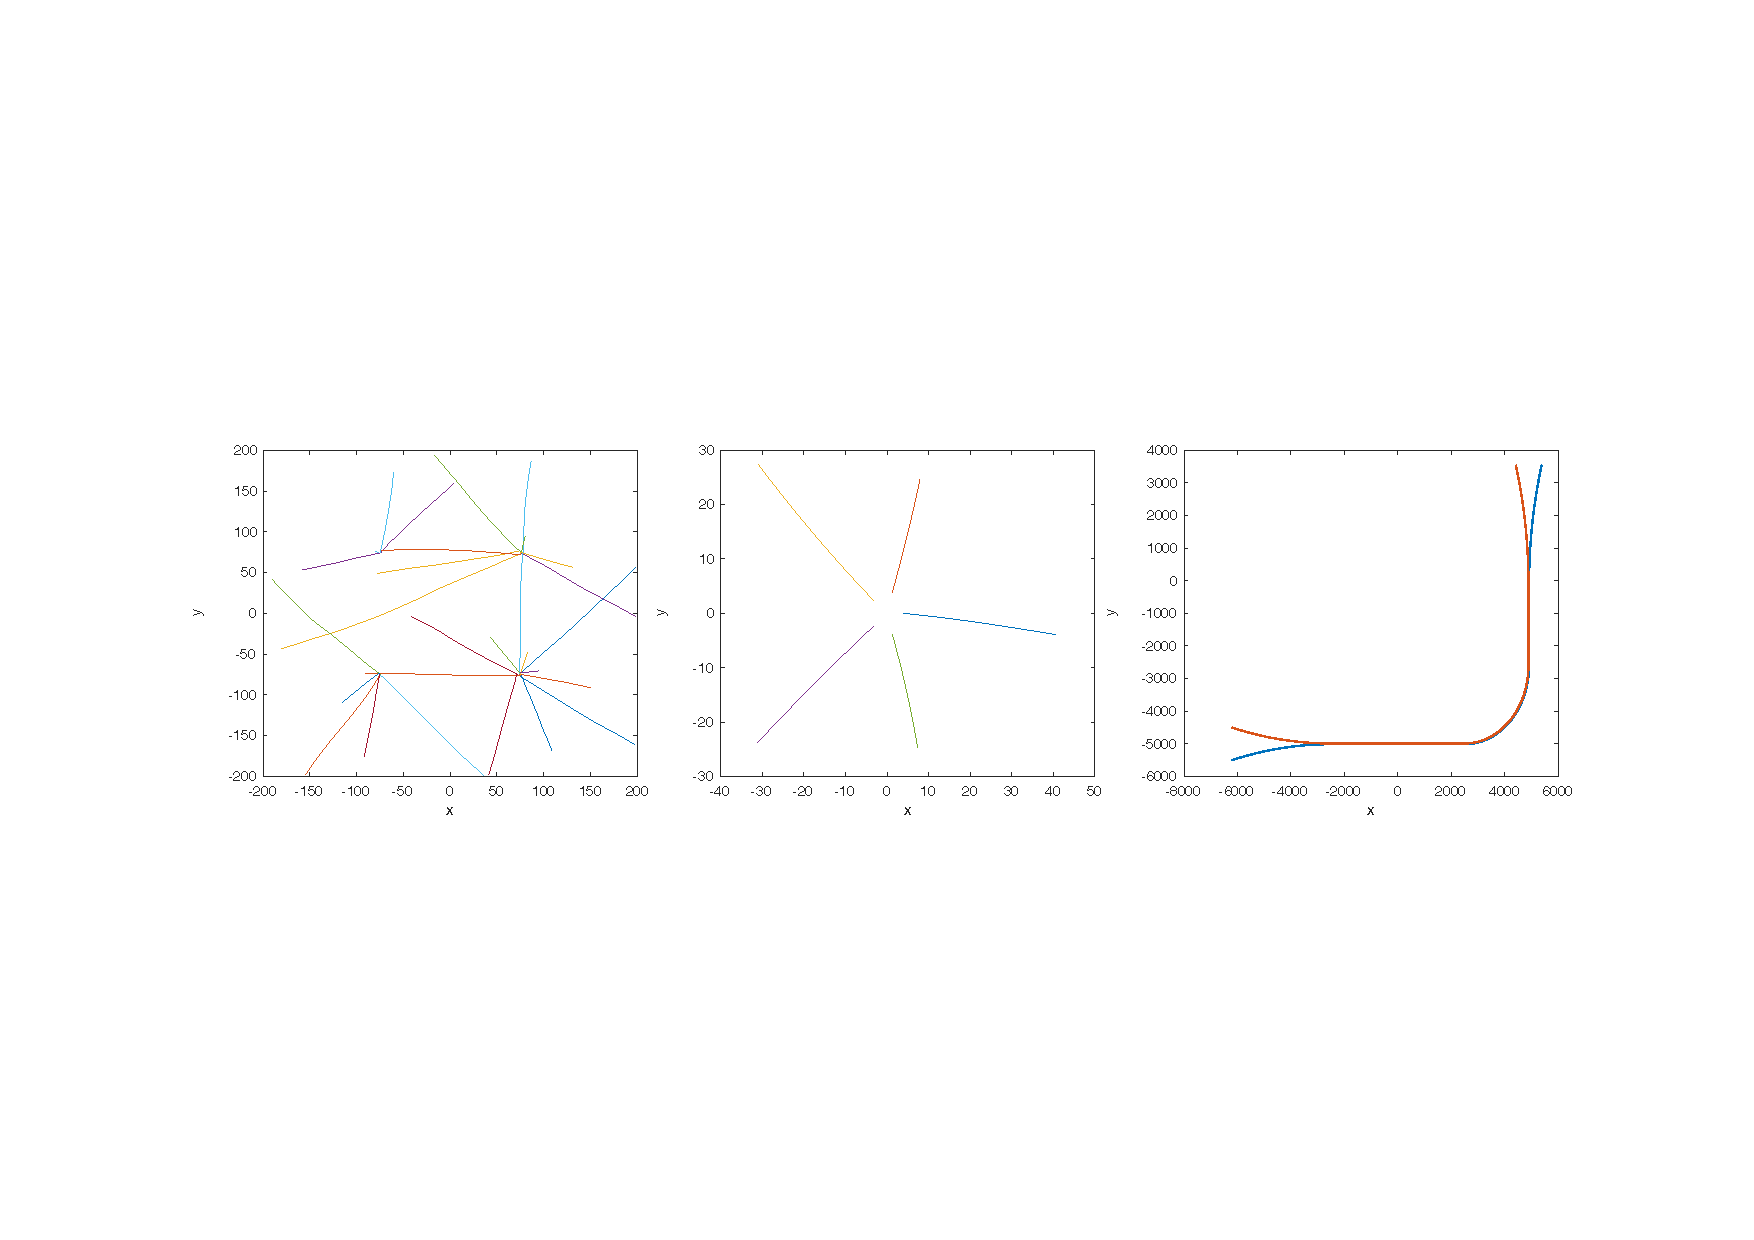
\includegraphics[width=0.48\textwidth]{trajectory}
\caption{True target trajectories of three scenarios, from left to right: 1) 27 objects, 2) dense birth, and 3) parallel manoeuvre.}
\label{fig:trajectory}
\end{figure}
\begin{table}[!b]
\caption{Average time $[s]$ to run one full Monte Carlo simulation}
\label{tab:CycleTimes}
	\centering
	\begin{tabular}{c | l l l l}
		Scenario & PHD & PMBM & PMB w/ OA & PMB w/ EAFS  \\
		\hline
		1   & $34.1$ & $57.6$ & $37.9$ & $41.1$ \\
		2 & $21.4$ & $45.8$ & $7.7$ & $8.5$ \\
		3 & $92.0$ & $41.4$ & $25.5$ & $25.1$
	\end{tabular}
\end{table}
\begin{figure*}[!t]
	\centering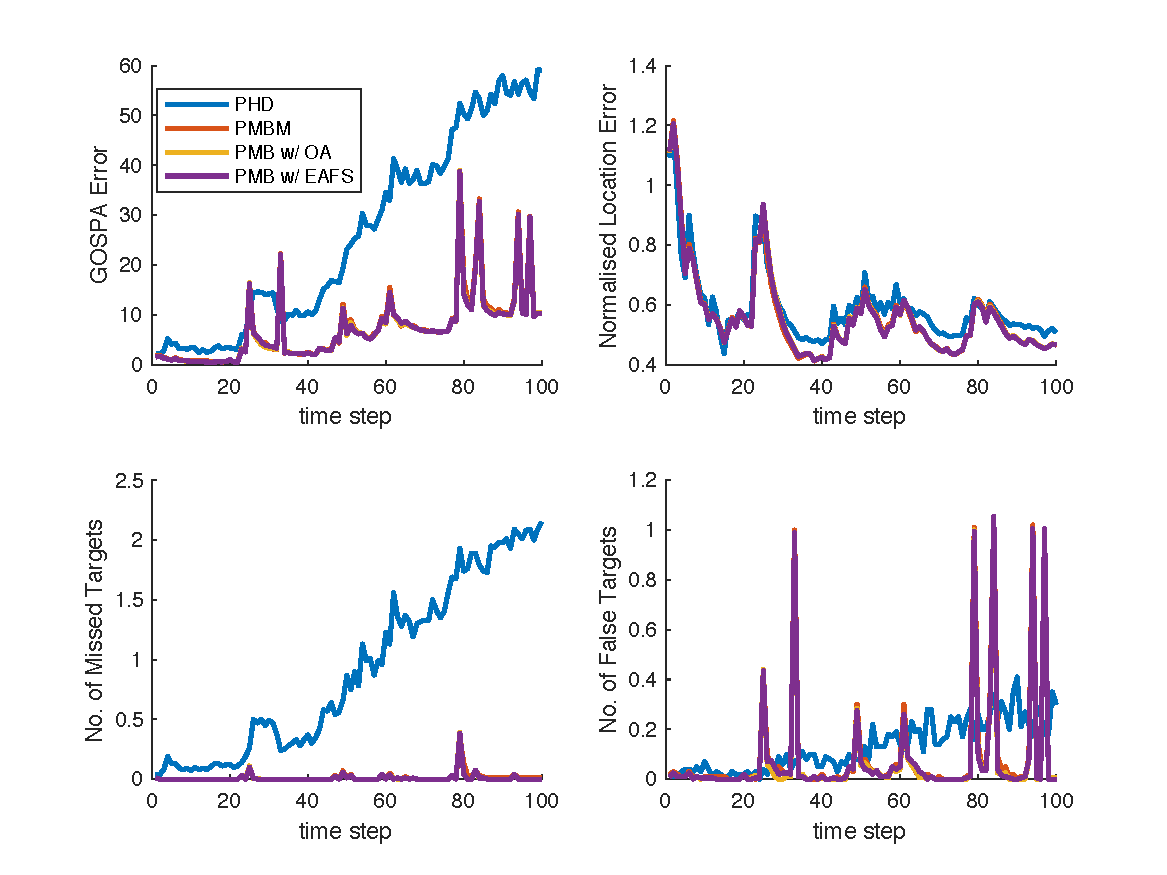
\includegraphics[width = 0.67\columnwidth]{GOSPA27Targets}
	\hspace{-2mm}
	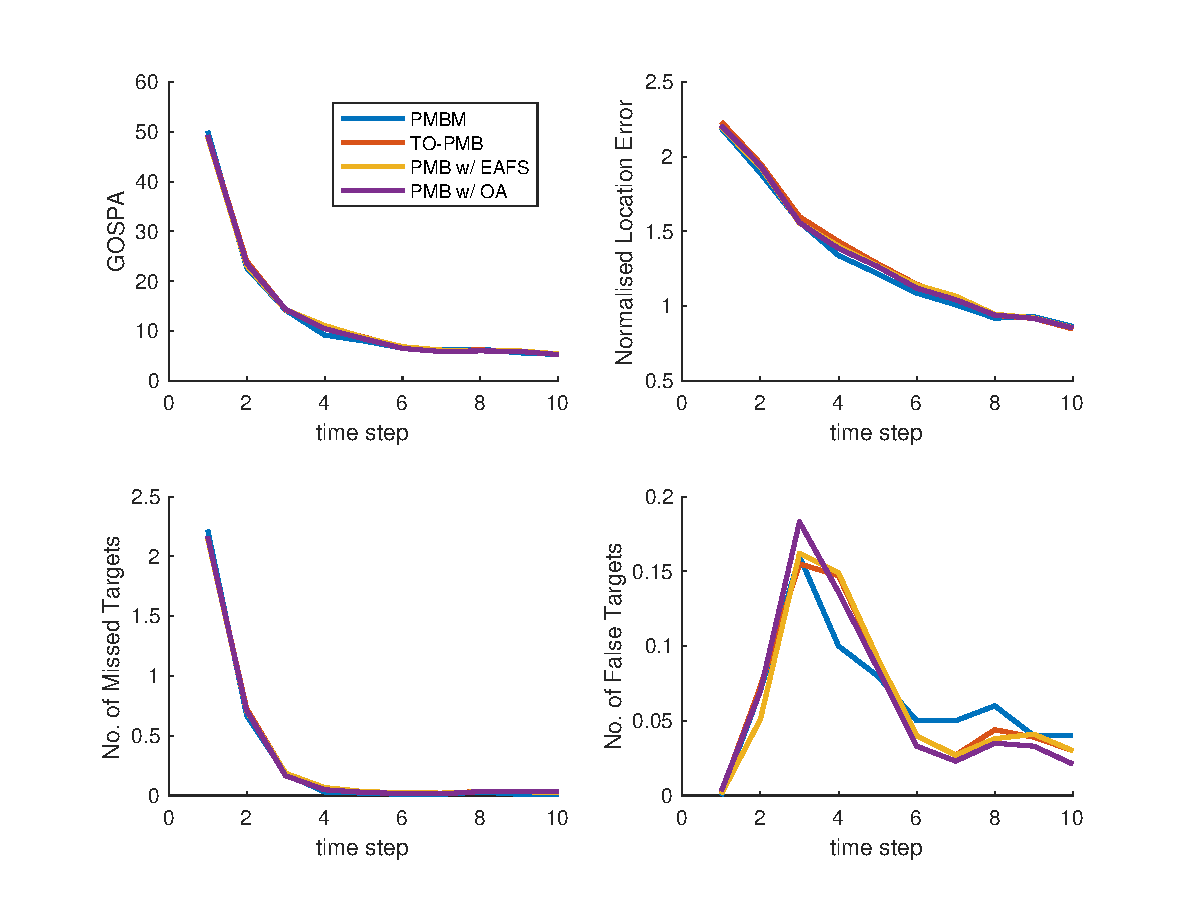
\includegraphics[width = 0.67\columnwidth]{GOSPAdenseBirth}
	\hspace{-2mm}
	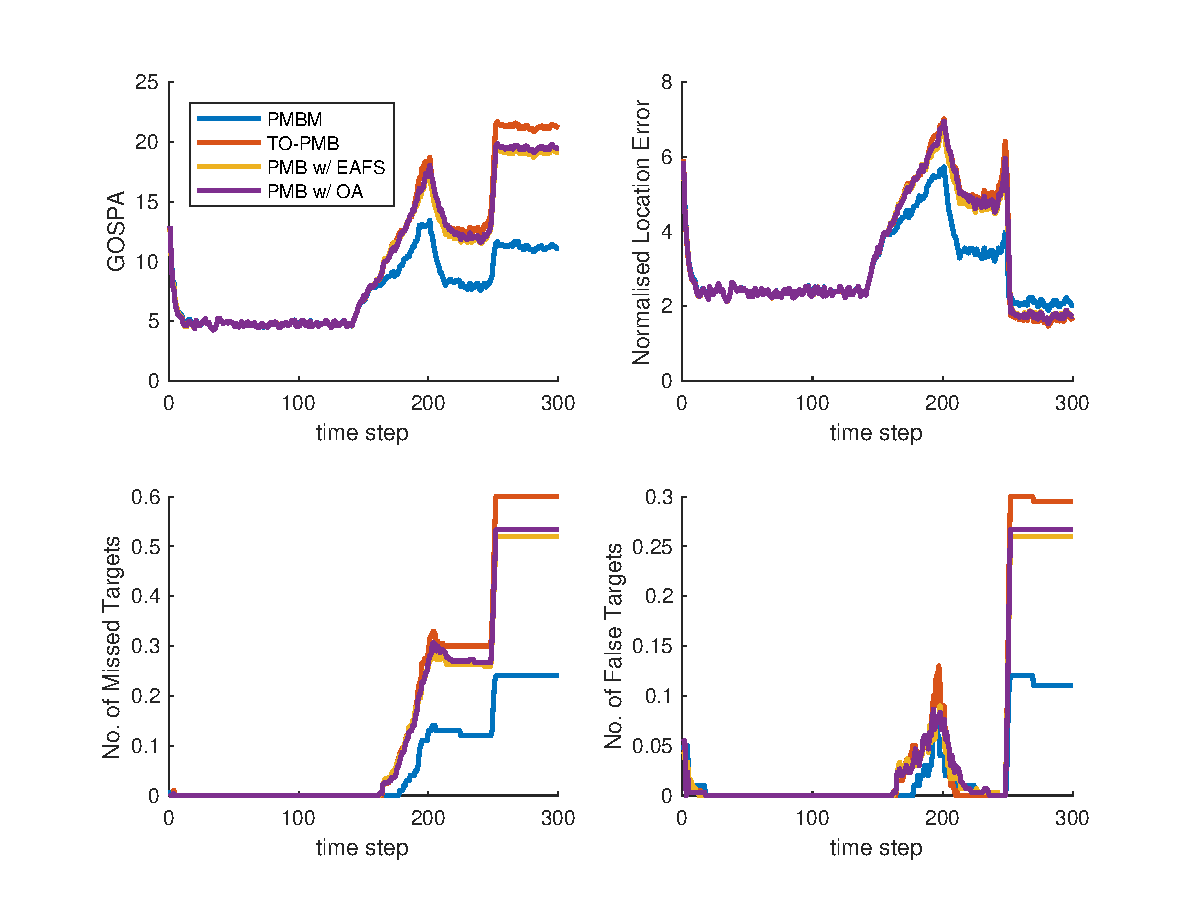
\includegraphics[width = 0.67\columnwidth]{GOSPAparallelTurn}
	\caption{Results from simulation of three scenarios, from left to right: 1) 27 objects, 2) dense birth, and 3) parallel manoeuvre.}%Overall \textsc{mhg} and \textsc{so} have best performance.
	\label{fig:SimulationResults}
\end{figure*}
In the first scenario, 27 randomly generated targets are born from four localised position, and they appear and disappear the surveillance area at different time steps. The parameters were set to $p^D = 0.90, p^S = 0.99$ and $ \lambda = 60$. This scenario illustrates how the different filters behave with a high target number and high clutter density scenario. In the second scenario, five targets are born at a very short distance from each other at the same time step. The parameters were set to $p^D = 0.90, p^S = 0.99$ and $ \lambda = 20$. This scenario tests different filters capabilities of handling dense birth. In the third scenario, two targets first get close, and then they manoeuvre in close proximity before splitting. The parameters were set to $p^D = 0.98, p^S = 0.99$ and $ \lambda = 10$. Here, the data association is very challenging due to coalescence and motion model mismatch.

% The scenario parameters clutter rate $\lambda$, detection probability $p^D$ , and survival probability $p^S$ are summarised in Table \ref{tab:SimulationParameters}.

The GOSPA performance of different filters is shown in Fig. \ref{fig:SimulationResults}, and the average times to run a single Monte Carlo trial of the three scenarios are given in Table \ref{tab:CycleTimes}. From the results of the simulation study, we see that filters based on MB conjugate priors have better performance than the PHD filter. The two variants of the PMB filter showed very similar performance in these three scenarios. The PMB filter has lower computational complexity than the PMBM filter with MBM merging, and the difference of average running time is most distinct in the scenario with dense birth. But the PMBM filter is able to produce better target extent estimations than the PMB filter especially in the scenario with parallel manoeuvre.
% True target trajectories for the three simulated scenarios. In scenario 1 (left), 27 targets are born from four localised positions, and they appear and disappear the area at different time steps. In scenario 2 (centre), five targets are born from roughly the same position at the same time. In scenario 3 (right), two targets first get close, and then they manoeuvre next to each other before splitting.



% \begin{table}
% \caption{Simulation scenario parameters}
% \label{tab:SimulationParameters}
% 	\centering
% 	\begin{tabular}{c | l l l}
% 		Scenario & $\lambda$ & $p^D$ & $p^S$\\
% 		\hline
% 		1 & $60$ & $0.90$ & $0.99$ \\
% 		2 & $20$ & $0.90$ & $0.99$ \\
% 		3 & $10$ & $0.98$ & $0.99$
% 	\end{tabular}
% \end{table}





\section{Conclusions}
This paper has proposed a tractable and efficient extended target filtering algorithm based on a PMBM conjugate prior approximation to the posterior density. A simulation study shows that the proposed PMB filter retains the advantage of the PMBM filter but with lower computational complexity. Possible future work includes how to improve the estimation of target extent and how to incorporate the formation of new tracks in the variational MB algorithm. 


\bibliographystyle{IEEEtran}
\bibliography{IEEEabrv,mybibli}


\end{document}
